\section{Other project outputs}
\label{sec:other_outputs}

\subsection{Predicting willingness to use thrombolysis from SSNAP organisational audit data}

We performed a multiple regression model to investigate whether organisational audit results reported by SSNAP could be used to predict a teams. The SSNAP Organisational Audit collects biennial data on the structure and organization of acute hospital stroke services, including bed numbers, staffing and seniority levels (including at the ‘front door’), models of delivery of hyperacute services including reperfusion, and other structural data. We devised a model to investigate whether organisational audit data reported by SSNAP could be used to predict a team’s propensity to use thrombolysis, as measured by the SHAP value for the stroke team in the thrombolysis decision model. We were not able to identify any significant predictors of ‘willingness to thrombolyse’ from these data, indicating that there were no features of the organisation of hyperacute staffing or other provision, including unit size and admission numbers, that were predictive of a site’s propensity to use thrombolysis (see \url{https://github.com/samuel-book/thrombolysis_organisational_factors/blob/main/data_prep/2c_statsmodels.ipynb}). This finding runs counter to the often-cited notion that sites with higher rates of thrombolysis tend to be those that are larger and better staffed. Evidence is clear that organisation factors do affect thrombolysis use \cite{carter-jones_stroke_2011}; we simply did not find a strong link between willingness to use thrombolysis and the organisational audit output. This could be due to the SSNAP Organisational Audit recording numbers from a single day snap shot, and more frequent data collection may enable identification of significant predictors of ‘willingness to thrombolyse’.

\subsection{Pilot thrombectomy model}

As part of this study we performed a pilot experiment on the effect of thrombectomy (mechanical removal of the clot) on outcomes in moderate-severe stroke (NIHSS 6+). The same model method was used as the outcome modelling with thrombolysis, but time from onset to thrombectomy was also added as an input feature. Figure \ref{fig:thrombectomy} shows the relationship between time from onset to thrombectomy. \textbf{These results have not been robustly investigated, and should be taken as indicative only}, but we saw a beneficial effect of thrombectomy. The beneficial effect of thrombectomy decayed over time; Early thrombectomy was able to significantly improve the odds of being discharged with mRS 0-2 (with this effect being in addition to the effect of thrombolysis). More work is required to confirm and better understand this effect, with the significantly larger number of patients who have received thrombectomy that is now in SSNAP.

\begin{figure}[!h]
    \centering
    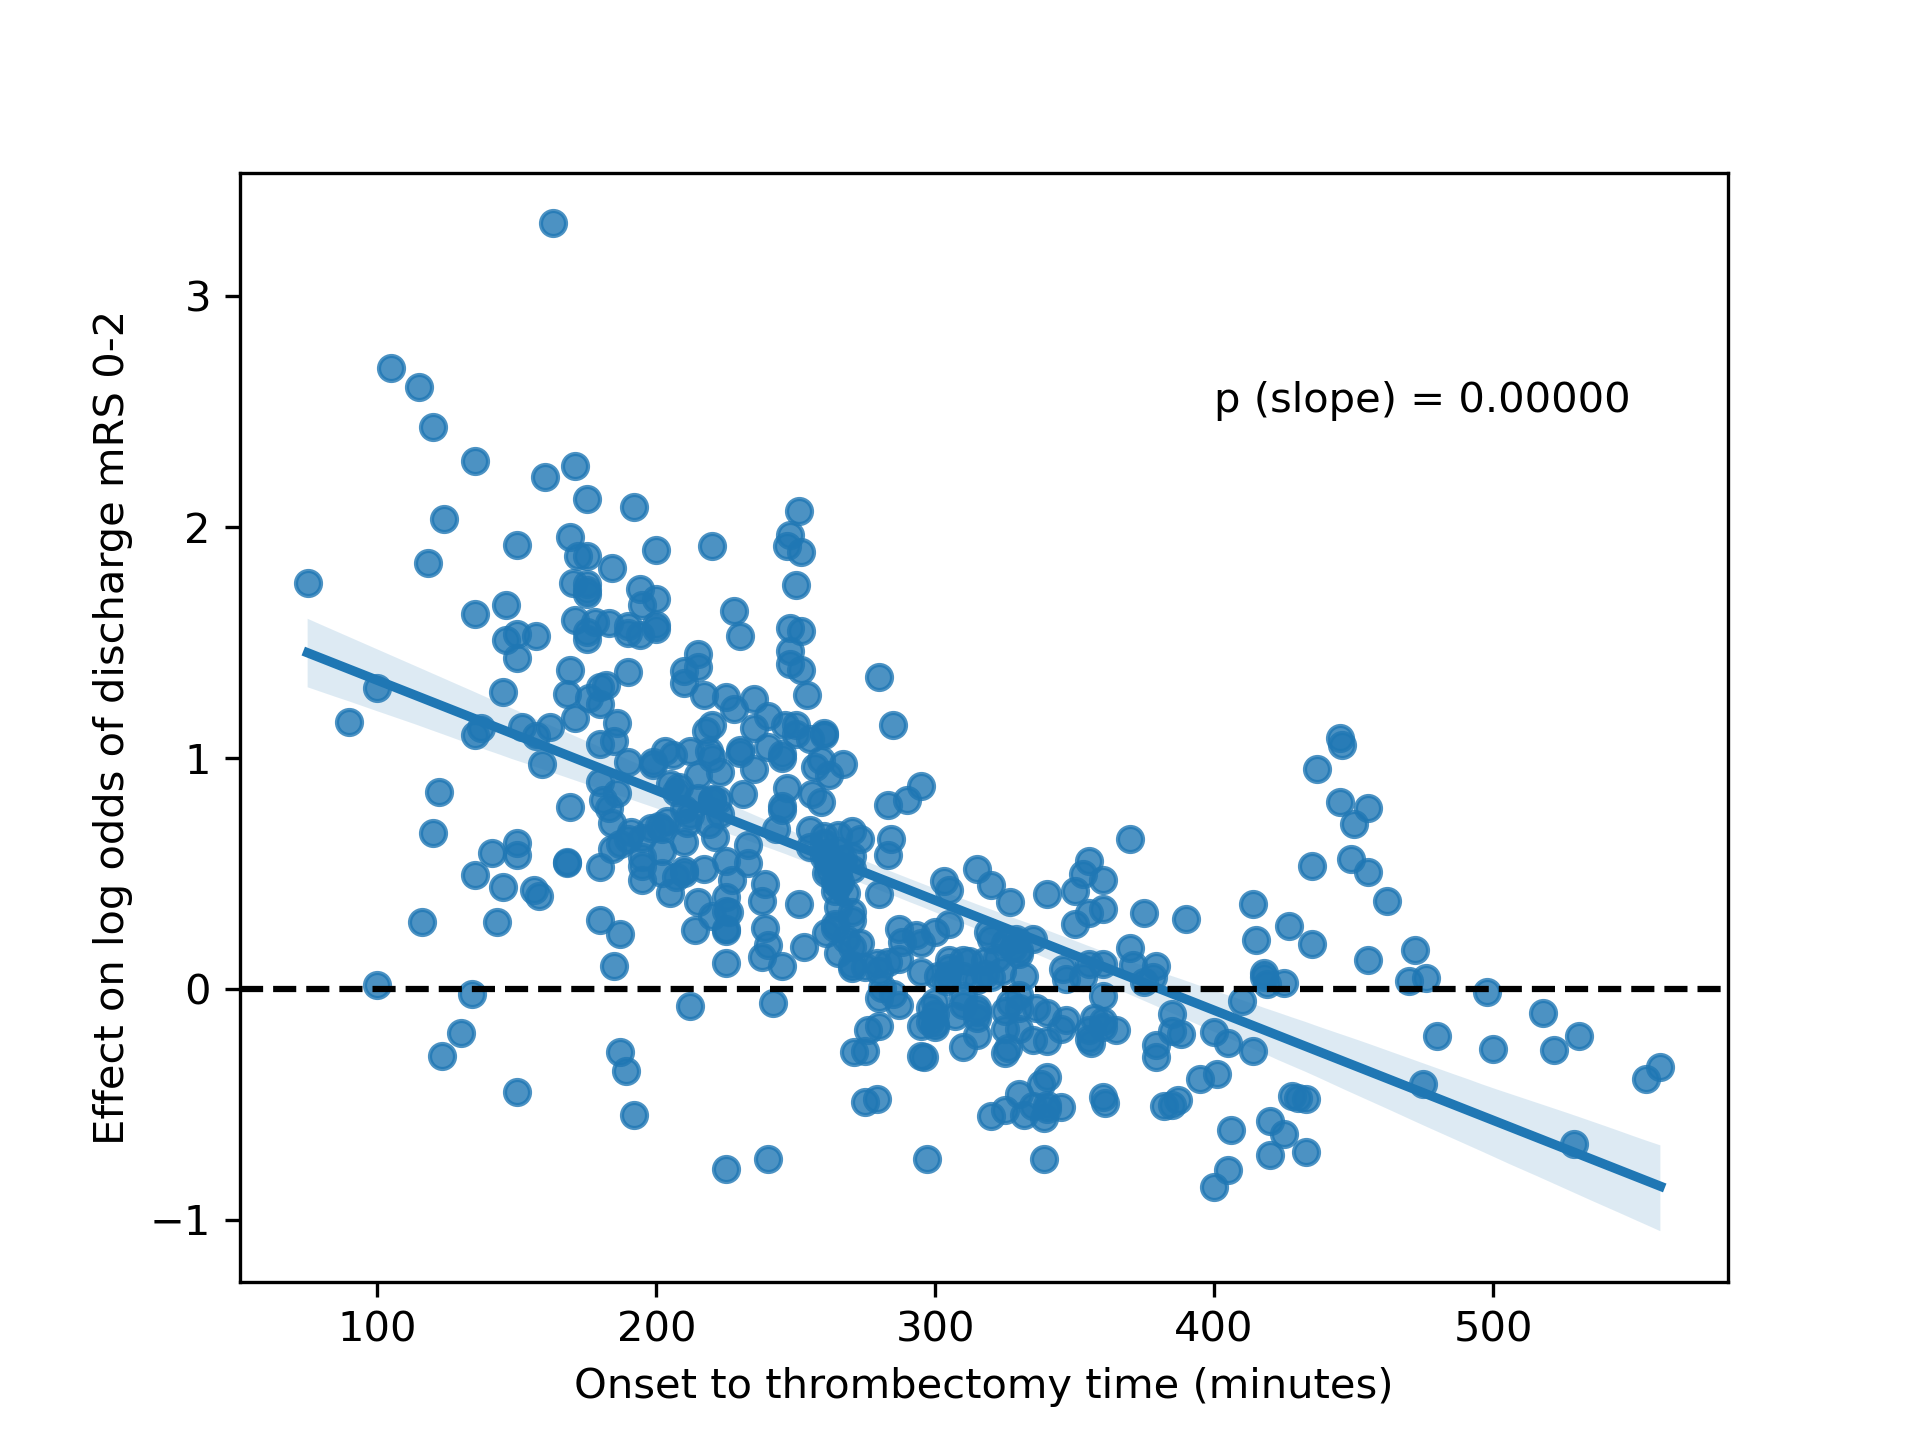
\includegraphics[width=0.6\linewidth]{images/thrombectomy}
    \caption{The effect of time of onset to thrombectomy on the log of odds of being discharged with mRS 0-2 for patients with stroke severity of NIHSS 6+ (using the SHAP value for the effect of thrombectomy). Data shown is for patients that received thrombectomy within 10 hours of stroke onset. This effect is the effect of thrombectomy in addition to any effect of thrombolysis. \textbf{Results show pilot work and should be taken as indicative only}.}
    \label{fig:thrombectomy}
\end{figure}



